\section{NP-hard}
In the previous chapter, we briefly discussed the definition of NP-hard problems as well as the academic significance of Sokoban as a proxy for solving generic NP-hard problems. This leads to the question of how Fryers et al.\ proved that Sokoban is NP-hard.

Before following their proof, we first define a $P$ problem as a problem that can be solved in at most polynomial time. $NP$ problems are ones for which the existence of a solution can be verified in polynomial time, though the solution itself cannot necessarily be derived that quickly. Any $P$ problem is in $NP$ because if we can derive a solution in polynomial time, we can also verify it in polynomial time. It is unknown whether all $NP$ problems are in $P$. $NP\text{-hard}$ problems are ones to which any other $NP$ problem can be reduced. An $NP\text{-hard}$ problem that is also in $NP$ itself is an $NP\text{-complete}$ problem. The simplest $NP\text{-complete}$ problem is the Boolean Satisfiability problem: for a given boolean expression $B(x_1,x_2,\ ...\ ,x_n)$ that includes $\neg$, $\land$, and $\lor$, is there an assignment of $x_1,x_2,\ ...\ ,x_n$ that makes $B$ true?

If Sokoban can answer this question, then the game is as hard as Boolean Satisfiability, which is an $NP\text{-hard}$ problem, and is therefore an $NP\text{-hard}$ problem itself. To establish this, the researchers first demonstrated that simple boolean expressions can be encoded as playable Sokoban levels; ``a level has a solution if and only if the expression can be true, and such that we can construct (in polynomial time) a valuation from a solution and vice versa'' \cite{fryers1995sokoban}. Successfully encoding a boolean expression that includes all of $\neg$, $\land$, and $\lor$ would show that Sokoban can express any propositional formula in this fragment.

\begin{figure}[h] % [h] forces the image to be placed "here"
    \centering
    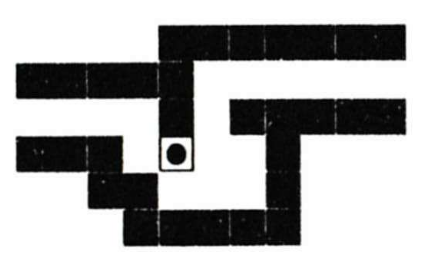
\includegraphics[width=0.3\textwidth]{images/nphard-1.png} 
    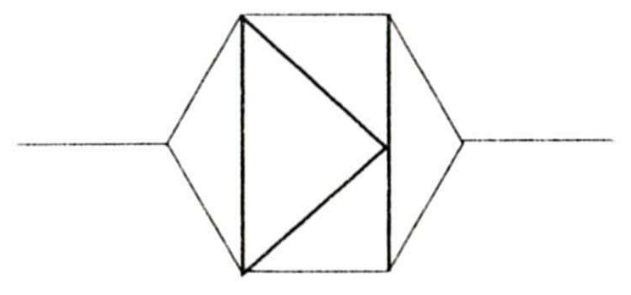
\includegraphics[width=0.3\textwidth]{images/nphard-5.png} 
    \caption{}\label{fig:nphard-1}
\end{figure}

Figure \ref{fig:nphard-1} shows a level with one entrance on the left and one exit on the right. The player can travel from the entrance to the exit by pushing the barrel (marked with a black circle) to the right and, after going through, back to the left in order to clear the path to the exit. Not only does this clear the path for the player, but it also places the barrel back on the goal position, marked with a square. However, the player cannot travel from the exit to the entrance because the player can only push the box to the left, which would block the path and render the box immobile. This structure is called a \textit{turnstile}.

\begin{figure}[h] % [h] forces the image to be placed "here"
    \centering
    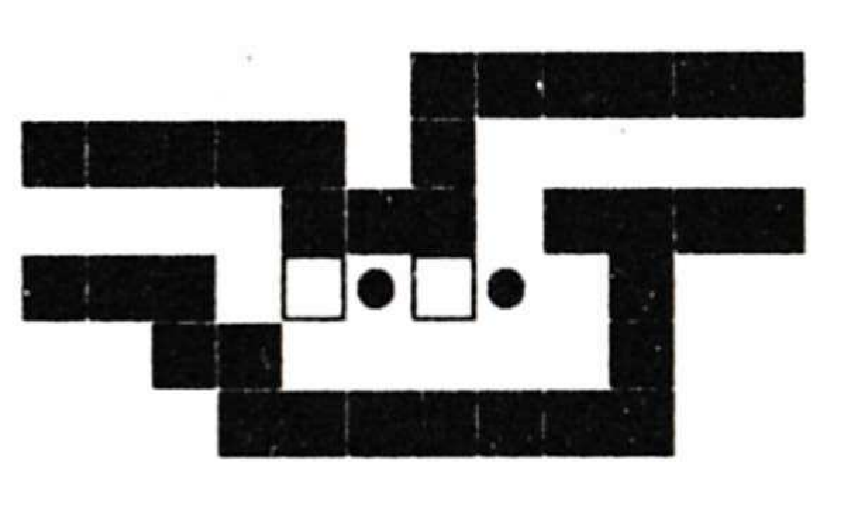
\includegraphics[width=0.3\textwidth]{images/nphard-2.png} 
    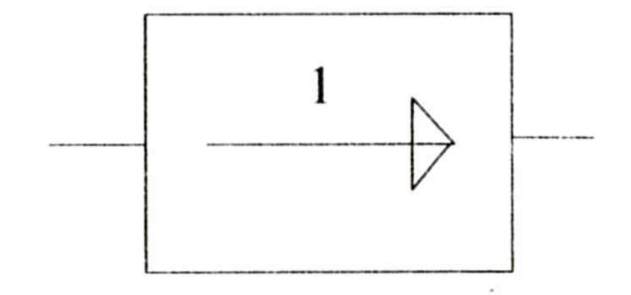
\includegraphics[width=0.3\textwidth]{images/nphard-6.png} 
    \caption{}
    \label{fig:nphard-2}
\end{figure}

Figure \ref{fig:nphard-2} shows a \textit{1-gate} that can only be traveled once by the player, and only in one direction, from left to right. This is because the left barrel needs to be pushed to the left to its goal position to be considered solved, and this action must precede the movement of the right barrel, which, after its push to the left, would prevent the left barrel from being moved. This gate can be placed in parallel to create an \textit{n-gate}, which allows traversal from left to right $n$ times.

Using a combination of $n\text{-gates}$ and $turnstiles$, we will construct the following boolean expression:
$$B(x,y,z) = (z\ \land\ \{(\neg y\ \land \neg z) \lor (\neg x\ \lor y)\})$$

\begin{figure}[h] % [h] forces the image to be placed "here"
    \centering
    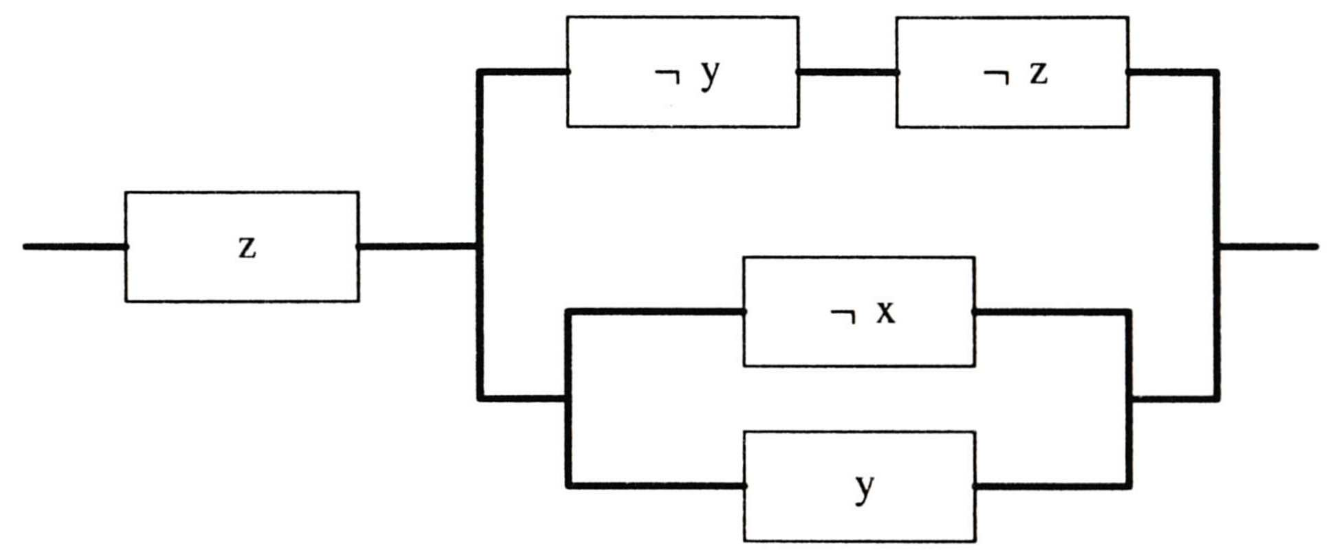
\includegraphics[width=0.8\textwidth]{images/nphard-3.png} 
    \caption{}
    \label{fig:nodegraph}
\end{figure}

The same boolean expression can be expressed as a graph of nodes (Figure \ref{fig:nodegraph}) where the player can only travel from left to right. 

For a given set of $x,y,z$, each node is traversable only if the expression inside is true. 

If the player can start from the left-end of the graph and reach the right-end of the graph, $B(x,y,z)$ is true. 

For example, if $x=0,y=0,z=1$, it would go through the nodes $z$ and $ \neg x$ to reach the right-end of the graph. 

This graph can then be recreated with the previous Sokoban level sections if we define each node as following:

\begin{figure}[h] % [h] forces the image to be placed "here"
    \centering
    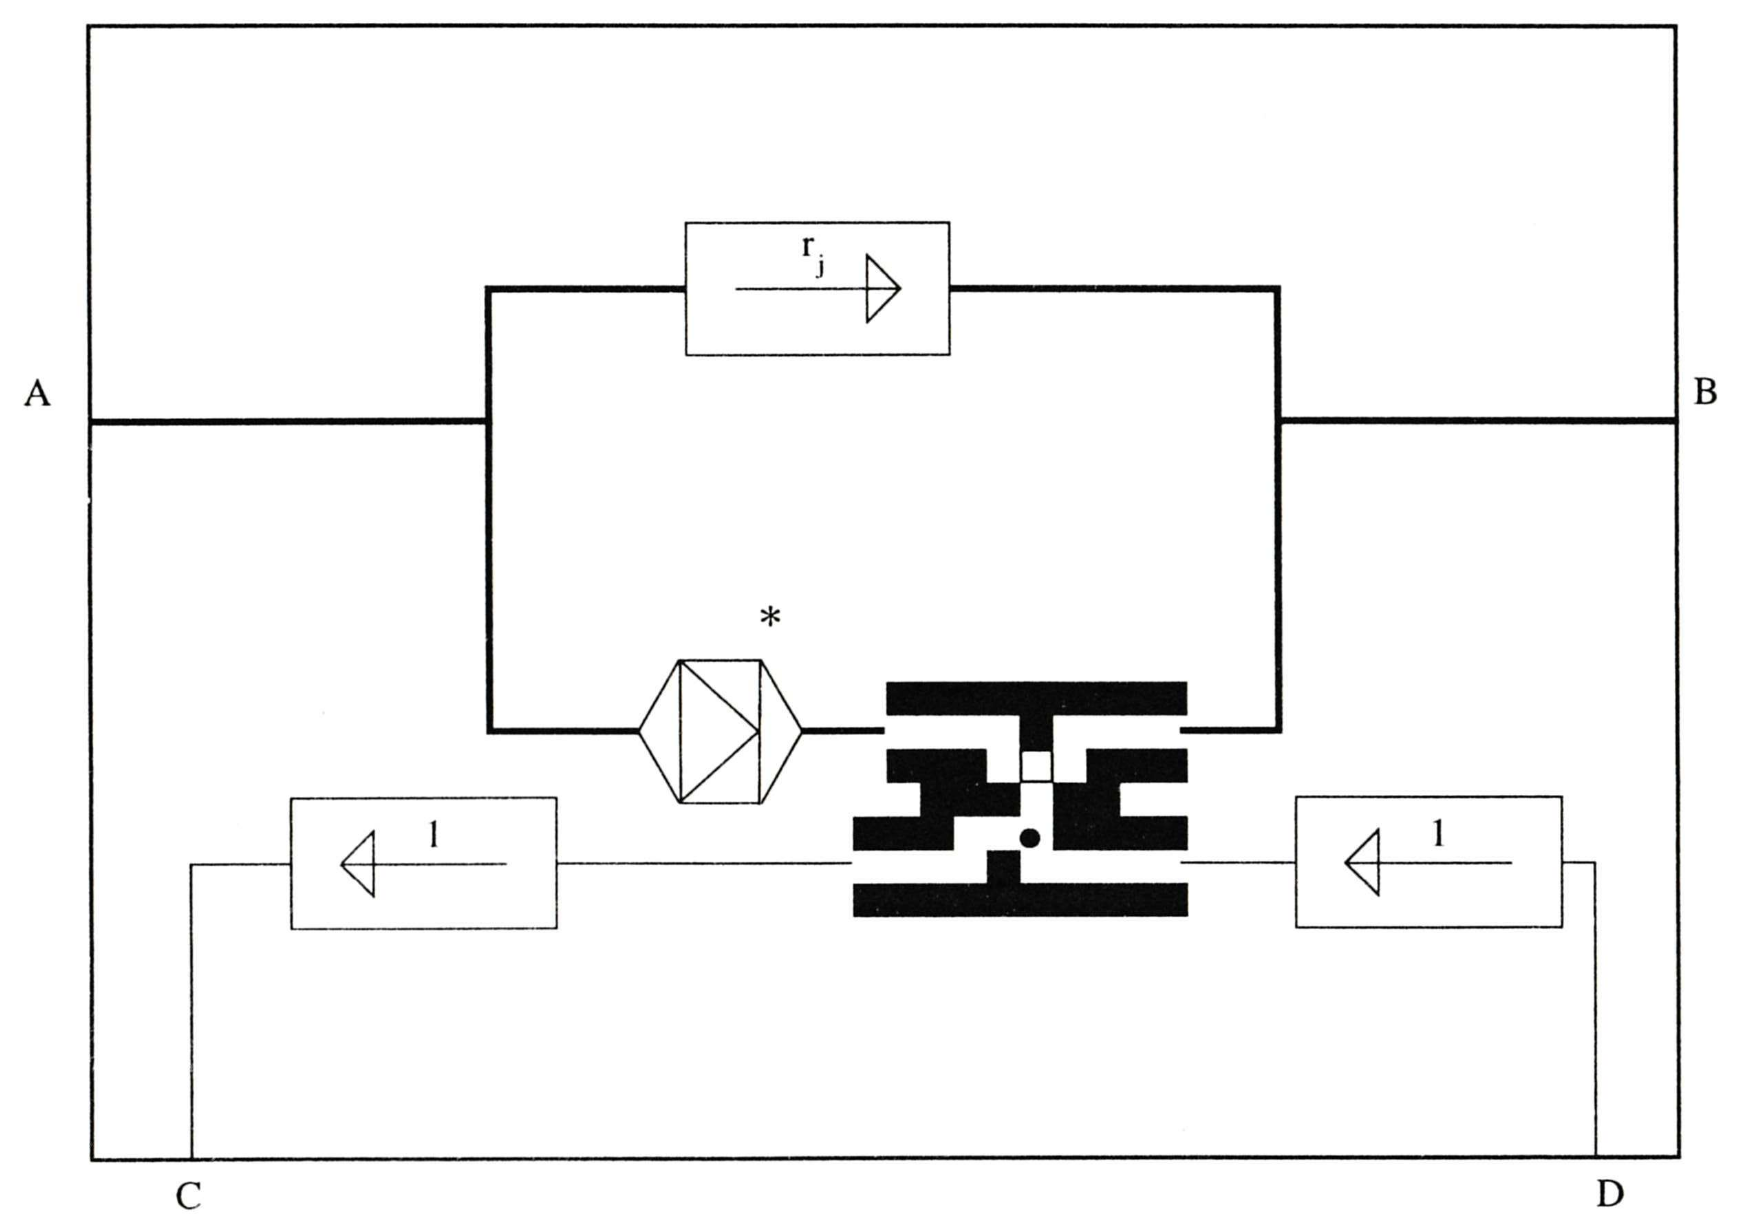
\includegraphics[width=0.8\textwidth]{images/nphard-4.png} 
    \caption{}
    \label{fig:nphard-4}
\end{figure}

The node has entrances $A,D$ and exits $B,C$. The player can traverse the node on the bold line through either the $r_j\text{-gate}$ (an $n\text{-gate}$ that can be traveled through $r_j$ times) or the $turnstile$. Notice that if the player enters $D$ and leaves through $C$, it blocks the $turnstile$ path above and forces the player to go through the $r_j\text{-gate}$ path, as the barrel will be pushed upwards into the $turnstile$ path and become stuck there. The bold path and the faint path are separate because, even though the barrel can be pushed away, it would cause the barrel to get stuck in a non-goal position. This node will be incorporated into the node graph from Figure \ref{fig:nodegraph} in a way that blocks the bold path of the $x$ node when $x=0$, blocks $\neg y$ when $y=1$, and so on.

To show that $B$ has a solution, the player has to be able to complete the node graph implemented in Sokoban shown in Figure \ref{fig:b_implementation}. (Figure \ref{fig:b_implementation} also uses a crossover implemented in Sokoban, which is omitted in this paper for brevity.)

Suppose $B(x,y,z)$ as implemented in Figure \ref{fig:b_implementation} is true (solvable with all barrels on their goal positions) and there exists a set of inputs $(x_1,x_2,\ ... , x_n)$ (which is $x,y,z$ in our expression) that makes $B$ true. With this condition, the player can solve $B$ by following the steps below:

\begin{enumerate}
    \item From `start', travel the path $x$ if $x$ is true and $\neg x$ otherwise, and so on.
    \item The player reaches P for the first time. From here, travel the bold paths using the $turnstile$ path of each node without using the $r_j\text{-gates}$, which can be done because $B$ is true. The player reaches Q.
    \item Traverse the faint paths not used in the first cycle to return to P.
    \item From P, use the bold paths to reach Q, using the $r_j\text{-gates}$ of the set of nodes that connect P to Q.
    \item The player has now fully solved the path between `start' and P. The remaining combinations of the bold paths that connect P to Q can be traveled by using the bottom bold line that has no node.
    \item After traveling through the $(r+1)\text{-gate}$ $r+1$ times, the player can place the barrel in the R section to complete the entire level.
\end{enumerate}

This demonstrates that Sokoban can successfully encode an $NP\text{-hard}$ problem and is therefore an $NP\text{-hard}$ problem itself. Readers can choose to complete Figure \ref{fig:b_implementation} by hand with the truth table below:

\begin{table}[h]
\centering
\label{tab:sokoban_logic}
\renewcommand{\arraystretch}{1.2} % Adds breathing room between rows
\begin{tabular}{ @{} ccc | ccc | cc | c | c @{} }
\toprule
$x$ & $y$ & $z$ & $\neg x$ & $\neg y$ & $\neg z$ & $\neg y \land \neg z$ & $\neg x \lor y$ & Inner Term & $B(x,y,z)$ \\
\midrule
0 & 0 & 0 & 1 & 1 & 1 & 1 & 1 & 1 & 0 \\
0 & 0 & 1 & 1 & 1 & 0 & 0 & 1 & 1 & 1 \\
0 & 1 & 0 & 1 & 0 & 1 & 0 & 1 & 1 & 0 \\
1 & 0 & 0 & 0 & 1 & 1 & 1 & 0 & 1 & 0 \\
\addlinespace % Visual break for readability
0 & 1 & 1 & 1 & 0 & 0 & 0 & 1 & 1 & 1 \\
1 & 0 & 1 & 0 & 1 & 0 & 0 & 0 & 0 & 0 \\
1 & 1 & 0 & 0 & 0 & 1 & 0 & 1 & 1 & 0 \\
\addlinespace % Visual break for readability
1 & 1 & 1 & 0 & 0 & 0 & 0 & 1 & 1 & 1 \\
\bottomrule
\end{tabular}
\caption{Truth table for the Boolean function $B(x,y,z)$}
\end{table}




\section{PSPACE-complete}
The preceding section established that Sokoban is an $NP\text{-hard}$ problem, following the proof of Fryers et al.\ \cite{fryers1995sokoban, cook2023complexity}. In addition to being an NP-hard game, Sokoban was also found to be PSPACE-complete \cite{culberson1997sokoban}. A PSPACE problem is a decision problem that can be solved by a Turing machine using a polynomial amount of memory space. If every problem in PSPACE can be reduced to a given problem $X$, then $X$ is PSPACE-hard. A problem is PSPACE-complete if and only if it is in PSPACE and is PSPACE-hard.

Culberson demonstrated that Sokoban is a PSPACE-complete problem by recreating a finite-tape Turing machine in Sokoban \cite{culberson1997sokoban}. To create the emulator, the researcher relied on two basic properties of the game. The first is the notion of unrecoverable configuration. This is when it is not possible to move a box to its goal position, either because the box was placed in a dead-end location or because the goal position is impossible to reach due to its placement. The second is the fact that the player's movement is also bound by the geometry of the puzzle. Several gadgets are then introduced, similarly to the NP-hard proof. Each gadget is a section of a Sokoban puzzle. These gadgets are combined into Cellular Units, each representing one cell of the finite Turing machine's tape. Culberson proves that the puzzle created from these Cellular Units has a solution if and only if the emulated Turing machine halts in an ``accept'' state.


\section{Automatic Generation of Sokoban Puzzles}
One of the earliest subsequent strands of academic research on Sokoban focused on generating Sokoban puzzles. The researchers framed the work as an attempt to generate art with computers, arguing that the creation of art by computer is an important target of artificial intelligence \cite{murase1996automatic}. Through the automatic generation of Sokoban puzzles, Murase et al.\ laid the foundation for generating datasets for Sokoban agents \cite{murase1996automatic}.

\begin{figure}[!ht] % [h] forces the image to be placed "here"
    \centering
    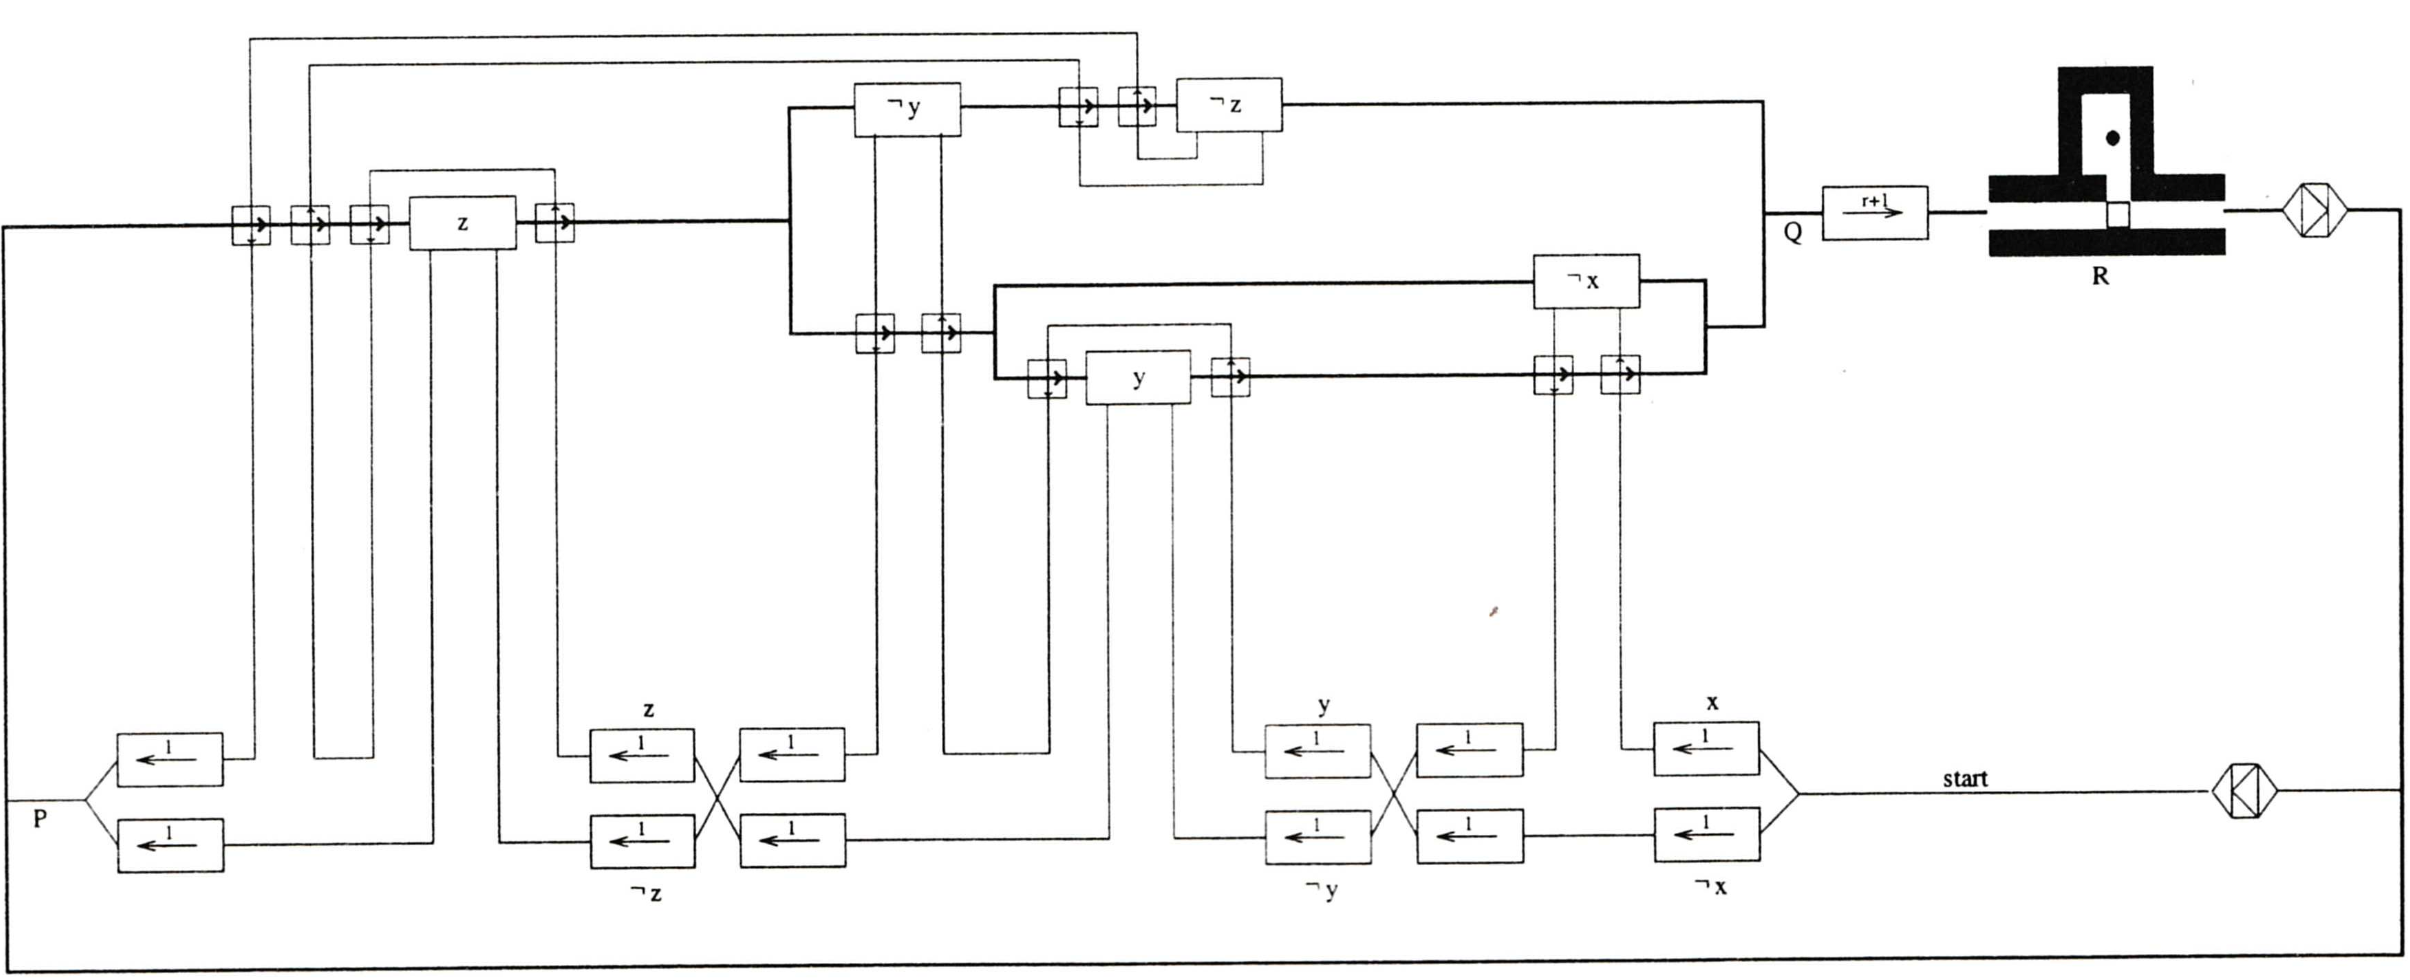
\includegraphics[width=1.2\textwidth, angle=90]{images/nphard-7.png} 
    \caption{}
    \label{fig:b_implementation}
\end{figure}

\begin{figure}[h] % [h] forces the image to be placed "here"
    \centering
    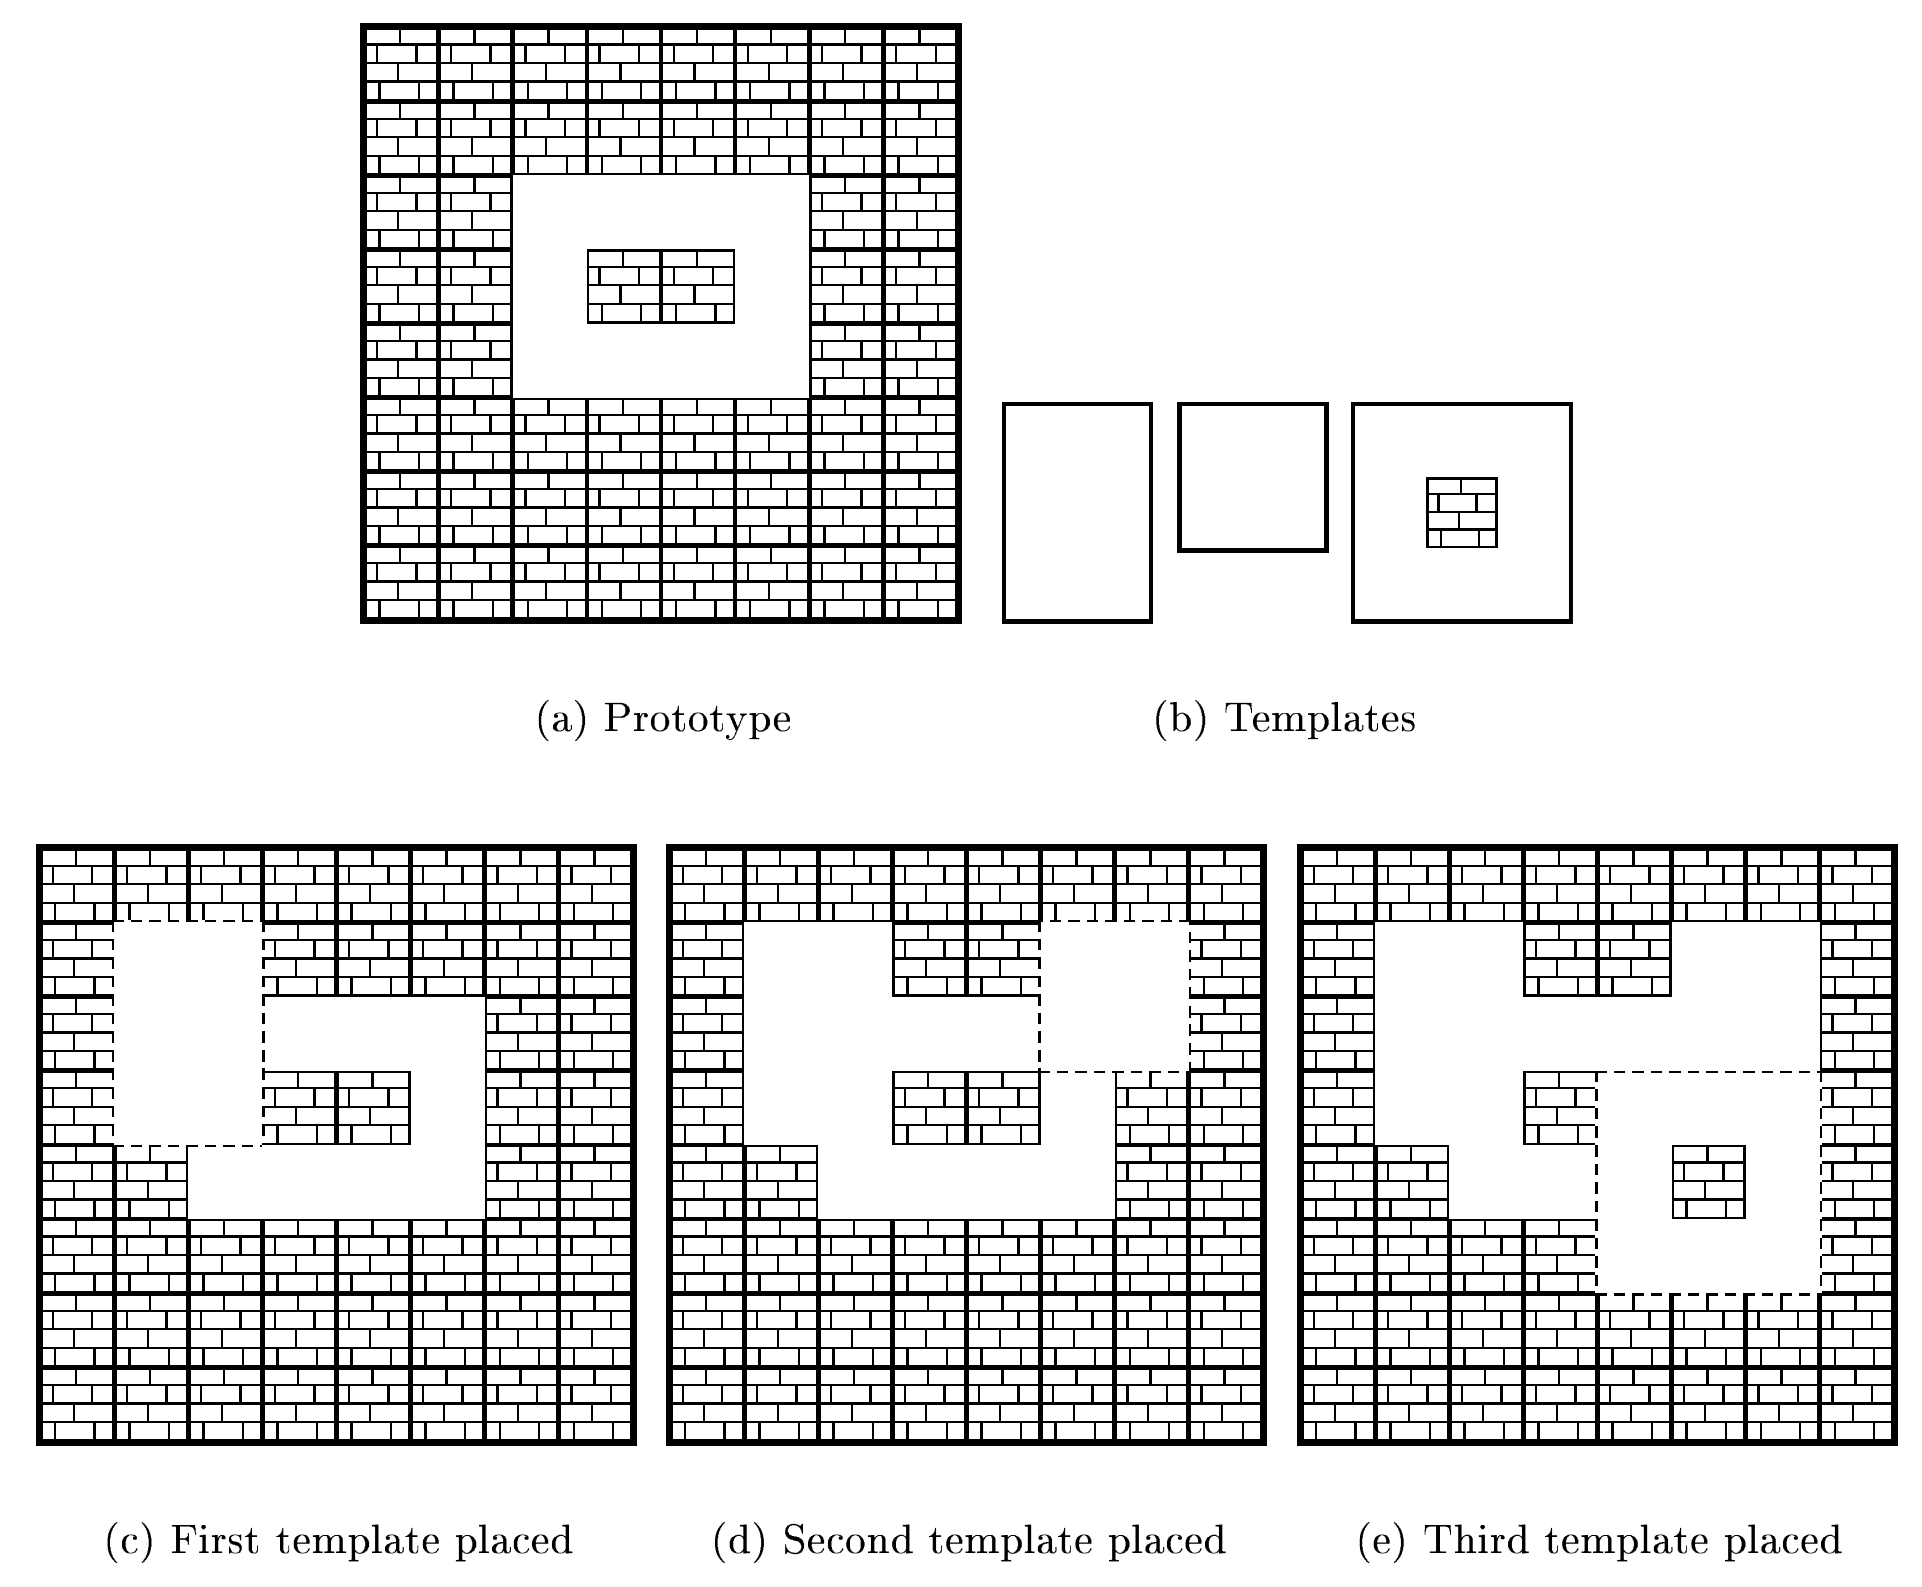
\includegraphics[width=0.9\textwidth]{images/autogeneration1.png}
    \caption{}
    \label{fig:ag1}
\end{figure}

The researchers achieved automatic generation of Sokoban levels through a three-step methodology. First, candidate problems are generated randomly from a prototype and three templates. Next, unsolvable candidates are removed by a Sokoban solver. Finally, trivial or uninteresting candidates are removed by the evaluator. Templates are $2\times 3$, $2\times 2$, and $3\times 3$ empty spaces, used to encourage the generation of multiple paths inside the space. After tiles are placed (Figure \ref{fig:ag1}), there are some tiles where a box can never be placed. These tiles are marked as GOAL\_AVOID (Figure \ref{fig:autogeneration2}). Goal-candidate tiles that are in corners are marked as COR\_GOAL, and the next goal is placed on goal-candidate tiles that are not dead ends and not COR\_GOAL. The dead-end ADD\_AVOID areas are recalculated after every placement.

After the generation of the level, a Breadth-First Search is used to solve the puzzle. While the BFS solver is not able to find solutions to puzzles with long sequences, it can still effectively search for solutions with short sequences \cite{fryers1995sokoban}. Puzzles that cannot be solved are pruned in this step.

The most crucial contribution of this paper is the metric used to determine whether a generated puzzle is non-trivial and interesting. The evaluation program aims to evaluate artistic value using the following criteria:

\begin{center}
    \begin{minipage}{0.8\textwidth} % Adjust width as needed
        \begin{itemize}
            \item Length of solution sequence: if a problem has a very short solution sequence, it is trivial and is rejected. When the length of a problem's solution sequence is less than seven, the problem is rejected.
            \item Number of changes in pushing direction during the solution sequence: in interesting problems, the keeper has to change the direction of pushing objects very often. If the number of changes is less than four, the problem is trivial and must be removed.
            \item Number of detours in the solution sequence: if a problem's solution sequence has no detours, it is uninteresting and is rejected.
        \end{itemize}
    \end{minipage}
\end{center}

The authors claim that these criteria guide the generation of interesting puzzles.


\begin{table}[ht]
    \centering 
    \begin{tabular}{|l|l|l|}
    \hline
    \multicolumn{2}{|l|}{\# of generation failures} & 7 \\ \hline
    \multicolumn{2}{|l|}{\# of problems that have no solutions} & 245 \\ \hline
    \multirow{2}{*}{solvable problems} & removed & 204 \\ \cline{2-3} 
    & outputted & 44 \\ \hline \hline
    \multicolumn{2}{|l|}{\# of trials} & 500 \\ \hline \hline
    \multicolumn{2}{|l|}{real good problems} & 14 \\ \hline
    \end{tabular}
    \caption{Experimental results of the automatic Sokoban generator \cite{murase1996automatic}.}
    \label{table:2}
\end{table}

\begin{figure}[h] % [h] forces the image to be placed "here"
    \centering
    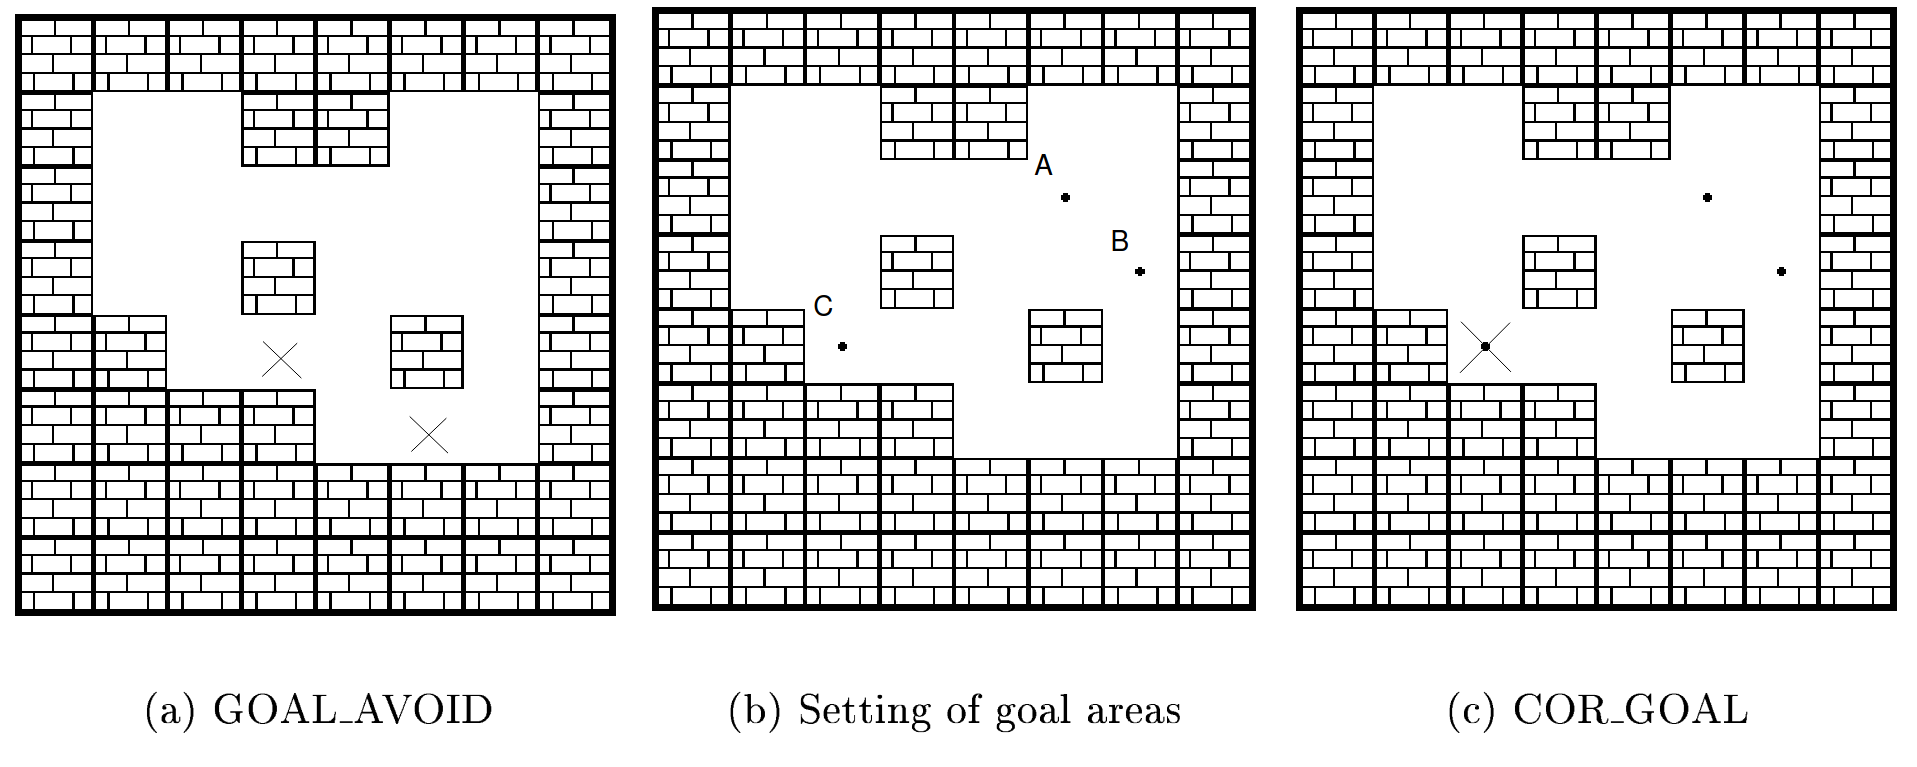
\includegraphics[width=0.9\textwidth]{images/autogeneration2.png} 
    \caption{}
    \label{fig:autogeneration2}
\end{figure}


\section{Early Attempts at Solving Sokoban}


In the late 90s and 2000s, the focus of Sokoban research shifted from the difficulty of the problem to the solution of the problem. Early attempts at solving Sokoban relied on variations of traiditional algorithmic search such as A*. Junghanns et al presented numerous research projects that in the late 90s. In one of their works, they attempt to solve all 90 puzzles of the XSokoban test suite using IDA*. \cite{myers_xsokoban} \cite{junghanns1997sokoban} \cite{junghanns1998sokoban} The researchers demonstrate a modified IDA* search method named 'Rolling Stone' that incorporates a Deadlock Table to identify a deadend circumstatance earlier in the heuristics search tree expansion to prune searching. The Deadlock Table consisted of 22 million entries of frequently occuring board pattern that leads to a deadend. The Rolling Stone also introduced a concept of 'Macro Moves' that collapses a sequence of forced moves into single steps for more efficient memory use during search while presercing solution optimality. 

The Rolling Stone algorithm was able to find solution to 16 problems out of 90 problems with a tree shallower than the solution itself. This was made possible with Macro Moves. However this method comes with significant limitation as it requires 22 million rows of deadlock pattern which is hard-coded domain knowledge. The paper also recognizes that the Rolling Stone spends 90\% of its execution time updating the lower bounds which means most of the processing time is spent on optimizing a found solution. \cite{junghanns1998sokoban} 

A similar method was tried by Pereira et al \cite{pereira2013finding} where researchers employ pattern database, a pre-computed lookup table that stores the shortest distances for simplified local problems, to be used as heuristics in the IDA* search. The authors introduced a concept called instance decomposition. Because it's not possible to know which stone is placed on which goal position before the solution of the puzzle, instance decompoisition assigns each stone to a specific goal before running the search. This constraint acts as an intermediate goal and converts the multi-goal problem into a single-goal problem. During the search, the Pattern Database provides an admissible heuristics to be used for pruning search tree. 



This motivates the search for better heuristics and representations.




3.6 — Reinforcement Learning Approaches
This is where the field pivots. The key papers:

Schrader (2018) — "Sokoban for OpenAI Gym" — created the standard RL benchmark environment most modern work uses.
Weber et al. / DeepMind (2017) — "Imagination-Based Planning" — used Sokoban as a testbed for model-based RL.
Guez et al. (2019) — "An Investigation of Model-free Planning" — DeepMind's direct attack on Sokoban with RL, showing its difficulty as a benchmark.


3.7 — Egocentric / Representation-Based Approaches
This is where you position your own work. You'd discuss how the representation of the state given to the agent affects learning — egocentric views vs. global views — which directly motivates your thesis contribution.

Cite Julieus Togelius \cite{togelius2005evolving} \cite{togelius2006evolving}
"These papers compared five controller architectures using egocentric (first-person), Newtonian (third-person), or no state information. The key finding was that the only controller able to evolve good behavior was the one based on a neural network acting on egocentric inputs. Wikipedia This is the canonical empirical demonstration that egocentric observation outperforms allocentric observation in evolved game agents."
\cite{risi2015neuroevolution}

"How to Frame This in Your Sokoban Thesis
The Togelius car racing result is your theoretical anchor for why you're trying egocentrism in Sokoban. The argument flows naturally: if egocentric representation was the decisive factor in evolved car racing controllers, it's worth investigating whether the same holds for a puzzle-solving agent in Sokoban, where the player's local context (what's immediately adjacent) may matter more than global board awareness. That's your research question."